\subsection{Real Data}
We now present the results of running the algorithm on several real
datasets. Two of the merchants had moderate-sized relation graphs with
about $10^5$ vertices and $10^6$ input edges (candidate
recommendations); the remaining merchants (3, 4 and 5) have on the
order of $10^6$ vertices and $10^7$ input edges between them. 
We estimated an upper bound on the optimum solution by taking the minimum of
$|L|c/a$ and the number of vertices in $R$ of degree at least
$a$. Figures~\ref{fig:real_a=1},~\ref{fig:real_a=2}
and~\ref{fig:real_a=3} plot the average of the optimality
percentage of the sampling, greedy and partition algorithms across all
the merchants respectively. Note that we could only run the partition
algorithm for the first two merchants due to memory constraints. \vs

\begin{figure}[t]
\centering
\begin{minipage}[h]{0.48\textwidth}
\centering
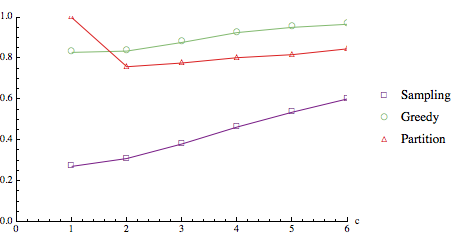
\includegraphics[width=0.8\textwidth]{images/real_a=1.png}
\caption{Real data runs when a=1}\label{fig:real_a=1}
\end{minipage}
\hspace{0cm}
\begin{minipage}[h]{0.48\textwidth}
\centering
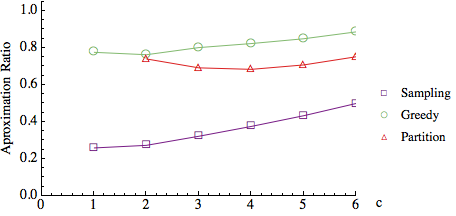
\includegraphics[width=0.8\textwidth]{images/real_a=2.png}
\caption{Real data runs when a=2}\label{fig:real_a=2}
\end{minipage}
\hspace{0cm}
\centering
\begin{minipage}[h]{0.48\textwidth}
\centering
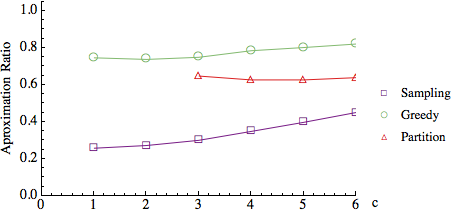
\includegraphics[width=0.8\textwidth]{images/real_a=3.png}
\caption{Real data runs when a=2}\label{fig:real_a=3}
\end{minipage}
\vspace{-0.2in}
\end{figure} \vs

From these results, we can see that that greedy performs exceptionally
well when $c$ gets even moderately large.  For the realistic value of
$c=6$, the greedy algorithm produced a solution that was 85\% optimal
for all the merchants we tested. For several of the merchants, its
results were almost optimal starting from $a=2$. \vs

The partition method is also promising, especially when the $a$ value
that is targeted is low. Indeed, when $a=1$ or $a=2$, its performance
is comparable or better than greedy, though it is not as pronounced as
the simulations. However, for larger values of $a$ the partition
algorithm performs worse. \vs

The sampling algorithm performs mostly well in real life data, but and
particularly so when $c$ is large. It is typically worse than
greedy, but unlike the partition algorithm, its performance improves
dramatically as $c$ becomes larger, and its performance does not get
worse as quickly when $a$ gets larger. Therefore, for large $c$ 
sampling becomes a viable alternative to greedy mainly in cases where the
linear memory cost of the greedy algorithm is too prohibitive. 
